\documentclass[12pt]{report}
\usepackage{amsmath}
\usepackage{graphicx}
\usepackage{hyperref}
\usepackage[utf8]{inputenc}
\usepackage{listings}

\title{CS3031 Advanced Telecommunications \\ Project I}
\author{Séamus Woods \\ 15317173}
\date{19/02/2019}

\begin{document}
\maketitle
\newpage


\section{Specification}
The objective of the excercise is to implement a Web Proxy Server. A Web proxy is a local server, which fetches items from the Web on behalf of a Web client instead of the client fetching them directly. This allows for caching of pages and access control.
\newline
\newline
The program should be able to:
\begin{itemize}
\item[1.] Respond to HTTP \& HTTPS requests, and should display each request on a management console. It should forward the request to the Web server and relay the response to the browser.
\item[2.] Handle websocket connections.
\item[3.] Dynamically block selected URLs via the management console.
\item[4.] Efficiently cache requests locally and thus save bandwidth. You must gather timing and bandwidth data to prove the efficiency of your proxy.
\item[5.] Handle multiple requests simultaneously by implementing a threaded server. 
\end{itemize}

\section{Implementation}
The easiest way to explain my design and implementation is just by talking through the execution of the code below. I have successfully managed to implement all features listed above. 
\newline
When the program is run, it will first start a thread on the tkinter function. Tkinter is what I used to dynamically block selected URLs(3).
\begin{center}
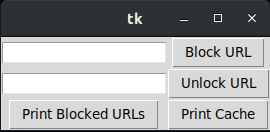
\includegraphics[scale=0.5]{tkinter.png}
\end{center}
As seen from the image, the user can dynamically enter URLs to be blocked, unblocked, can view the currently blocked URLs and print the URLs we currently have cached. This can all be done as the proxy is running(3).
\newline
The program then prompts the user to enter a port to have the proxy listen on. Once the user enters the port we initiate a socket, bind it to the port and start listening for incoming connections.
\begin{center}
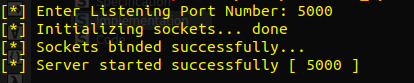
\includegraphics[scale=0.5]{beginning.png}
\end{center} 
Any connections we receive, we start a new thread on the proxy$\_$thread function with that specific connection, allowing multiple connections(5). 
\newline
In the proxy$\_$thread function we begin to parse the clients request. After some parsing to get the webserver, port, method etc, we check if we already have this page cached. If we do, we simply send the cached response the the client and we're done, else we call the proxy$\_$server function. (All of these requests are being timed and compared as part of the specification for caching(4)).
\newline
The first thing we do in our proxy$\_$server function is check our blocked url dictionary. If the webserver the client is trying to access is currently blocked, we simply tell them that that url is blocked and close the connection(3). 
\begin{center}
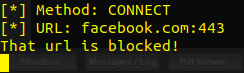
\includegraphics[scale=0.5]{blocked.png}
\end{center}
If the url is not blocked, we need to see if we are working with HTTP or HTTPS(1). If we are working with HTTPS the method should be CONNECT, and so we send the webserver a connection established. We then set up websocket connection(2) with the client and the webserver, which will persist until either of them end it. If we are working with HTTP, we don't need to worry about the CONNECT request, and just set up a websocket connection(2). As soon as we get the complete request, we store it in the cache, since we know it isn't there yet.  
\begin{center}
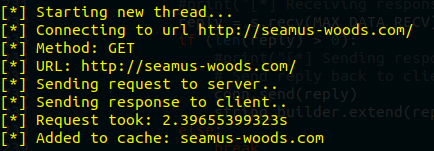
\includegraphics[scale=0.3]{beforecache.png}
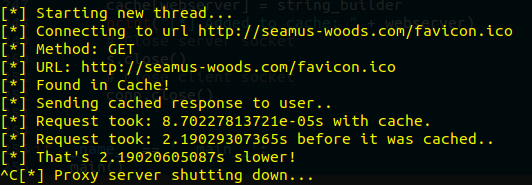
\includegraphics[scale=0.3]{aftercache.png}
\end{center}
The code can be seen below.


\section{Code}
\lstset{%
  language=Python,
  basicstyle=\footnotesize,
  showstringspaces=false,
  numbers=left,
  breakatwhitespace=false,
  breaklines=true,
  breakatwhitespace=true,
}
\lstinputlisting[language=Python]
{proxy.py}

\end{document}